\documentclass{article}
\usepackage[margin=0.75in]{geometry}
\usepackage{xcolor}
\usepackage{amsmath}
\usepackage{amssymb}
\usepackage{fontspec}
\usepackage{tikz}
\usetikzlibrary{tikzmark, arrows.meta, positioning, decorations.pathreplacing, calc}
\usepackage{enumitem}
\usepackage{multicol}

% ---------------------------------------------------------------------
%  THEME & COLORS
% ---------------------------------------------------------------------
\definecolor{bglight}{HTML}{FFFFFF}
\definecolor{textlight}{HTML}{000000}
\definecolor{subtext}{HTML}{666666}

% Model colors
\colorlet{redbar}{red!70!black}
\colorlet{bluebar}{blue!55!black}
\colorlet{greenbar}{green!60!black}
\colorlet{yellowbar}{yellow!80!black}

\pagecolor{bglight}
\color{textlight}
\pagestyle{empty}

% ---------------------------------------------------------------------
%  BUILDING BLOCKS
% ---------------------------------------------------------------------

% Circled step number.  \stepnum{number}{node-name}
\newcommand{\stepnum}[2]{%
  \tikzmarknode{#2}{%
    \begin{tikzpicture}[baseline=(char.base)]
      \node[draw=textlight, circle, inner sep=1.5pt, font=\sffamily\small] (char) {#1};
    \end{tikzpicture}%
  }%
}

% Dotted connectors between consecutive step nodes.
\newcommand{\stepchain}[1]{%
  \begin{tikzpicture}[remember picture, overlay]
    \def\prevnode{}%
    \foreach \n in {#1} {%
      \ifx\prevnode\empty\else
        \draw[dotted, thick, textlight!60] (\prevnode.south) -- (\n.north);%
      \fi
      \xdef\prevnode{\n}%
    }%
  \end{tikzpicture}%
}

% Worked-example steps
\newenvironment{steps}{\begin{description}[leftmargin=2em]}{\end{description}}

% Practice questions
\newenvironment{questions}[1][1]{%
  \begin{enumerate}[label=\textbf{\arabic*.}, start=#1, itemsep=2em, leftmargin=2em]%
}{\end{enumerate}}

% Headings
\newcommand{\examplehead}[1]{{\Large \textbf{Example: #1}}\par\vspace{0.5em}}
\newcommand{\practicehead}[1]{%
  \vspace{1em}\noindent\textcolor{subtext!40}{\rule{\linewidth}{0.5pt}}\vspace{1.5em}\par
  {\Large \textbf{#1}}\par\vspace{1em}}

% Answer blanks
\newcommand{\blank}[1][1.5cm]{\underline{\hspace{#1}}}
\newcommand{\ans}[1]{{\color{subtext}#1}}

\newcommand{\working}[2]{%
  $\begin{aligned}[t] #1 &= \blank[3cm] \\ &= \blank[3cm] \\ &\vphantom{#2}\end{aligned}$}

% ---------------------------------------------------------------------
%  BAR-MODEL HELPERS  (use inside tikzpicture)
% ---------------------------------------------------------------------
\newcommand{\bbar}[5]{%
  \draw[fill=#4, draw=black, line width=0.5pt] (#1,#3) rectangle (#2,{#3+0.5});
  \node[font=\small, text=white] at ({(#1+#2)/2},{#3+0.25}) {#5};}
\newcommand{\topbrace}[4]{%
  \draw[decorate, decoration={brace, amplitude=4pt}, line width=0.5pt] (#1,#3) -- (#2,#3);
  \node[anchor=south, font=\small] at ({(#1+#2)/2},{#3+0.1}) {#4};}
\newcommand{\botbrace}[4]{%
  \draw[decorate, decoration={brace, amplitude=4pt, mirror}, line width=0.5pt] (#1,#3) -- (#2,#3);
  \node[anchor=north, font=\small] at ({(#1+#2)/2},{#3-0.1}) {#4};}

% ---------------------------------------------------------------------
%  BASE-10 BLOCK HELPERS (Flats = Hundreds, Rods = Tens, Units = Ones)
% ---------------------------------------------------------------------
% \bflat{x}{y}  Draws a 100-flat (1.5cm x 1.5cm grid)
\newcommand{\bflat}[2]{%
  \draw[fill=redbar!15, draw=black, line width=0.4pt] (#1,#2) rectangle ++(1.5,1.5);
  \foreach \i in {1,...,9} {
    \draw[line width=0.2pt, subtext!40] (#1+\i*0.15,#2) -- ++(0,1.5);
    \draw[line width=0.2pt, subtext!40] (#1,#2+\i*0.15) -- ++(1.5,0);
  }%
}
% \brod{x}{y}   Draws a 10-rod (0.15cm x 1.5cm rod)
\newcommand{\brod}[2]{%
  \draw[fill=bluebar!25, draw=black, line width=0.4pt] (#1,#2) rectangle ++(0.15,1.5);
  \foreach \y in {1,...,9} {
    \draw[line width=0.2pt, subtext!40] (#1,#2+\y*0.15) -- ++(0.15,0);
  }%
}
% \bunit{x}{y}  Draws a 1-unit cube (0.15cm x 0.15cm)
\newcommand{\bunit}[2]{%
  \draw[fill=yellowbar!60, draw=black, line width=0.4pt] (#1,#2) rectangle ++(0.15,0.15);
}

% =====================================================================
\begin{document}
\sffamily

% ================= HEADER =================
\begin{center}
  {\Huge \bfseries Introduction to SG Math} \\[0.4em]
  {\Large \textcolor{subtext}{Base-Ten Blocks, Bar Models \& Mental Math Strategies}}
\end{center}
\vspace{1em}

% =====================================================================
%  PART 1 -- Friendly Numbers
% =====================================================================
\section*{Part 1: Friendly Numbers}

\noindent\textbf{Example 1 (Compatible Numbers):} Solve \textbf{$128 + 245 + 273 + 155 + 27 + 72$} by grouping friendly pairs.
\vspace{0.4em}

\begin{steps}
  \item[\stepnum{1}{p4s1}] \textbf{Identify compatible pairs}\\[0.2em]
  Look at the ones and tens digits to pair numbers that make whole hundreds:
  \\[0.4em]
  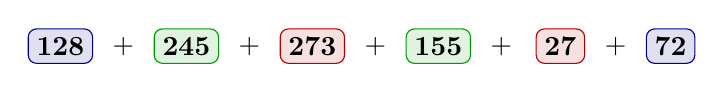
\begin{tikzpicture}[baseline={(0,0.1)}]
    \node[draw=bluebar, fill=bluebar!12, rounded corners=3pt, inner sep=3pt, font=\bfseries] at (0,0) {128};
    \node at (0.8,0) {+};
    \node[draw=greenbar, fill=greenbar!12, rounded corners=3pt, inner sep=3pt, font=\bfseries] at (1.6,0) {245};
    \node at (2.4,0) {+};
    \node[draw=redbar, fill=redbar!12, rounded corners=3pt, inner sep=3pt, font=\bfseries] at (3.2,0) {273};
    \node at (4.0,0) {+};
    \node[draw=greenbar, fill=greenbar!12, rounded corners=3pt, inner sep=3pt, font=\bfseries] at (4.8,0) {155};
    \node at (5.6,0) {+};
    \node[draw=redbar, fill=redbar!12, rounded corners=3pt, inner sep=3pt, font=\bfseries] at (6.35,0) {27};
    \node at (7.05,0) {+};
    \node[draw=bluebar, fill=bluebar!12, rounded corners=3pt, inner sep=3pt, font=\bfseries] at (7.75,0) {72};
  \end{tikzpicture}
  \vspace{0.3em}

  \item[\stepnum{2}{p4s2}] \textbf{Rearrange and group the pairs}\\[0.2em]
  \[ (128 + 72) + (245 + 155) + (273 + 27) \]

  \item[\stepnum{3}{p4s3}] \textbf{Add the friendly round hundreds}\\[0.2em]
  \[ 200 + 400 + 300 = \mathbf{900} \]
\end{steps}
\stepchain{p4s1,p4s2,p4s3}

\vspace{0.4em}

\practicehead{Practice Questions}

\begin{questions}
  % Question 1: 4-term compatible pairs
  \item \textbf{Pair compatible numbers to make hundreds, then solve:}

  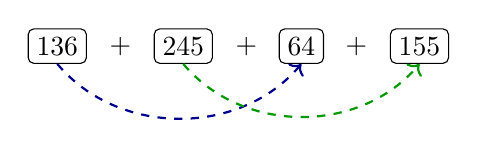
\begin{tikzpicture}[baseline={(0,0.1)}]
    \node[draw=black, rounded corners=2pt, inner sep=3pt] (q1) at (0,0) {136};
    \node at (0.8,0) {+};
    \node[draw=black, rounded corners=2pt, inner sep=3pt] (q2) at (1.6,0) {245};
    \node at (2.4,0) {+};
    \node[draw=black, rounded corners=2pt, inner sep=3pt] (q3) at (3.1,0) {64};
    \node at (3.8,0) {+};
    \node[draw=black, rounded corners=2pt, inner sep=3pt] (q4) at (4.6,0) {155};
    \draw[dashed, bluebar, thick, ->] (q1.south) to[out=-50, in=-130] (q3.south);
    \draw[dashed, greenbar, thick, ->] (q2.south) to[out=-50, in=-130] (q4.south);
  \end{tikzpicture}

  \vspace{0.4em}
  Equation: $(\blank + \blank) + (\blank + \blank) = \blank + \blank = \blank$

  % Question 2: 6-term compatible pairs
  \item \textbf{Rearrange into three compatible pairs to solve $118 + 265 + 234 + 135 + 66 + 82$:}

  \vspace{0.4em}
  Equation: $(\blank + \blank) + (\blank + \blank) + (\blank + \blank) = \blank + \blank + \blank = \blank$

  % Question 3: 4-term compatible pairs
  \item \textbf{Rearrange into compatible pairs to solve $345 + 182 + 155 + 218$:}

  \vspace{0.4em}
  Equation: $(\blank + \blank) + (\blank + \blank) = \blank + \blank = \blank$
\end{questions}
\pagebreak

% =====================================================================
%  PART 2 -- Rounding & Compensation
% =====================================================================
\section*{Part 2: Rounding and Compensation}

\noindent\textbf{Example 2 (Rounding \& Compensation):} Solve \textbf{$999 + 99 + 9$} using friendly benchmark numbers.
\vspace{0.4em}

\begin{steps}
  \item[\stepnum{1}{p4b1}] \textbf{Round up to the nearest powers of 10}\\[0.2em]
  Each number is just $1$ less than a round benchmark ($1000, 100, 10$):
  \\[0.4em]
  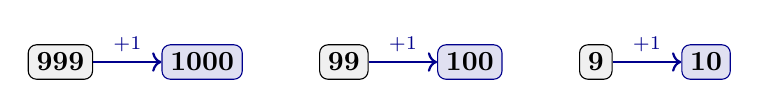
\begin{tikzpicture}[baseline={(0,0.1)}]
    \node[draw=black, fill=subtext!10, rounded corners=3pt, inner sep=3pt] (c1) at (0,0) {\textbf{999}};
    \node (b1) at (1.8,0) [draw=bluebar, fill=bluebar!12, rounded corners=3pt, inner sep=3pt] {\textbf{1000}};
    \draw[->, thick, bluebar] (c1) -- node[above, font=\scriptsize\bfseries] {$+1$} (b1);

    \node[draw=black, fill=subtext!10, rounded corners=3pt, inner sep=3pt] (c2) at (3.6,0) {\textbf{99}};
    \node (b2) at (5.2,0) [draw=bluebar, fill=bluebar!12, rounded corners=3pt, inner sep=3pt] {\textbf{100}};
    \draw[->, thick, bluebar] (c2) -- node[above, font=\scriptsize\bfseries] {$+1$} (b2);

    \node[draw=black, fill=subtext!10, rounded corners=3pt, inner sep=3pt] (c3) at (6.8,0) {\textbf{9}};
    \node (b3) at (8.2,0) [draw=bluebar, fill=bluebar!12, rounded corners=3pt, inner sep=3pt] {\textbf{10}};
    \draw[->, thick, bluebar] (c3) -- node[above, font=\scriptsize\bfseries] {$+1$} (b3);
  \end{tikzpicture}
  \vspace{0.3em}

  \item[\stepnum{2}{p4b2}] \textbf{Add the round numbers and track the total excess}\\[0.2em]
  We added $1 + 1 + 1 = 3$ extra, so we subtract $3$ from the round total:
  \[ (1000 + 100 + 10) - 3 = 1110 - 3 \]

  \item[\stepnum{3}{p4b3}] \textbf{Calculate the final sum}\\[0.2em]
  \[ 1110 - 3 = \mathbf{1107} \]
\end{steps}
\stepchain{p4b1,p4b2,p4b3}

\vspace{0.4em}

\practicehead{Practice Questions}

\begin{questions}
  % Question 1: Compensation with 9s
  \item \textbf{Use rounding and compensation to calculate $499 + 199 + 19$:}

  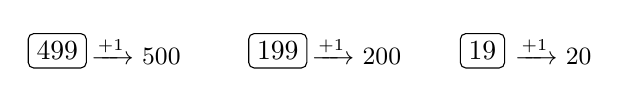
\begin{tikzpicture}[baseline={(0,0.1)}]
    \node[draw=black, rounded corners=2pt, inner sep=3pt] at (0,0) {499};
    \node at (1.0,0) [font=\small] {$\xrightarrow{+1}$ 500};
    \node[draw=black, rounded corners=2pt, inner sep=3pt] at (2.8,0) {199};
    \node at (3.8,0) [font=\small] {$\xrightarrow{+1}$ 200};
    \node[draw=black, rounded corners=2pt, inner sep=3pt] at (5.4,0) {19};
    \node at (6.3,0) [font=\small] {$\xrightarrow{+1}$ 20};
  \end{tikzpicture}

  \vspace{0.4em}
  Equation: $(\blank + \blank + \blank) - \blank = \blank - \blank = \blank$

  % Question 2: Compensation with 9s (unscaffolded)
  \item \textbf{Use rounding and compensation to calculate $599 + 299 + 89$:}

  \vspace{0.4em}
  Equation: $(\blank + \blank + \blank) - \blank = \blank - \blank = \blank$

  % Question 3: Compensation with numbers ending in 8
  \item \textbf{Use rounding and compensation to calculate $398 + 198 + 98$ (round each up by $+2$):}

  \vspace{0.4em}
  Equation: $(\blank + \blank + \blank) - \blank = \blank - \blank = \blank$
\end{questions}
\pagebreak

% =====================================================================
%  PART 3 -- Shifting (Subtraction Only)
% =====================================================================
\section*{Part 3: Shifting (Subtraction ONLY)}

\noindent
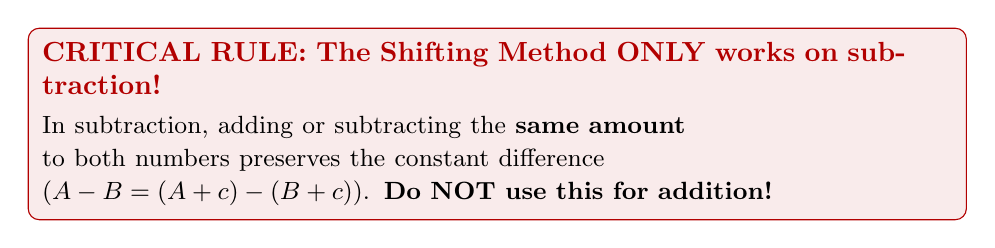
\begin{tikzpicture}
  \node[draw=redbar, fill=redbar!8, rounded corners=4pt, inner sep=5pt, text width=\dimexpr\linewidth-16pt\relax] {
    \textbf{\textcolor{redbar}{CRITICAL RULE: The Shifting Method ONLY works on subtraction!}} \\[0.2em]
    \small In subtraction, adding or subtracting the \textbf{same amount} to both numbers preserves the constant difference \linebreak ($A - B = (A + c) - (B + c)$). \textbf{Do NOT use this for addition!}
  };
\end{tikzpicture}
\vspace{0.5em}

\noindent\textbf{Example 3 (The Shifting Method for Subtraction):} Solve \textbf{$900 - 396$} by shifting to a round number.
\vspace{0.4em}

\begin{steps}
  \item[\stepnum{1}{p4c1}] \textbf{Identify the nearest round hundred}\\[0.2em]
  $396$ is only $4$ away from $400$.
  \vspace{0.2em}

  \item[\stepnum{2}{p4c2}] \textbf{Add the same amount ($+4$) to both numbers}\\[0.2em]
  Adding the same number to both terms preserves the difference (no borrowing across zeroes!):
  \\[0.4em]
  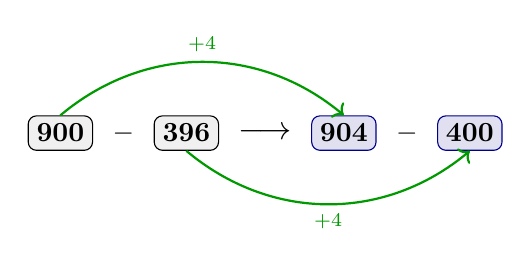
\begin{tikzpicture}[baseline={(0,0.15)}]
    \node[draw=black, fill=subtext!10, rounded corners=3pt, inner sep=3pt] (s1) at (0,0.3) {\textbf{900}};
    \node at (0.8,0.3) {$-$};
    \node[draw=black, fill=subtext!10, rounded corners=3pt, inner sep=3pt] (s2) at (1.6,0.3) {\textbf{396}};

    \node at (2.6,0.3) {\large $\longrightarrow$};

    \node[draw=bluebar, fill=bluebar!12, rounded corners=3pt, inner sep=3pt] (t1) at (3.6,0.3) {\textbf{904}};
    \node at (4.4,0.3) {$-$};
    \node[draw=bluebar, fill=bluebar!12, rounded corners=3pt, inner sep=3pt] (t2) at (5.2,0.3) {\textbf{400}};

    \draw[->, thick, greenbar] (s1.north) to[out=40, in=140] node[above, font=\scriptsize\bfseries, text=greenbar] {$+4$} (t1.north);
    \draw[->, thick, greenbar] (s2.south) to[out=-40, in=-140] node[below, font=\scriptsize\bfseries, text=greenbar] {$+4$} (t2.south);
  \end{tikzpicture}
  \vspace{0.3em}

  \item[\stepnum{3}{p4c3}] \textbf{Subtract without regrouping}\\[0.2em]
  \[ 900 - 396 = 904 - 400 = \mathbf{504} \]
\end{steps}
\stepchain{p4c1,p4c2,p4c3}

\practicehead{Practice Questions}

\noindent\textbf{Use the shifting method (constant difference) to make a round subtrahend:}
\vspace{0.4em}

\noindent
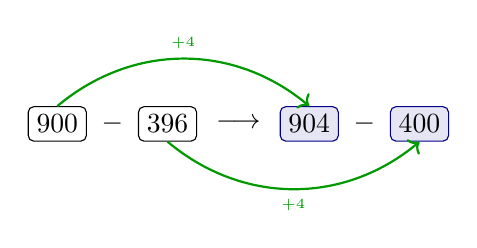
\begin{tikzpicture}[baseline={(0,0.1)}]
  \node[draw=black, rounded corners=2pt, inner sep=3pt] (sh1) at (0,0.2) {900};
  \node at (0.7,0.2) {$-$};
  \node[draw=black, rounded corners=2pt, inner sep=3pt] (sh2) at (1.4,0.2) {396};
  \node at (2.3,0.2) {$\longrightarrow$};
  \node[draw=bluebar, fill=bluebar!10, rounded corners=2pt, inner sep=3pt] (th1) at (3.2,0.2) {904};
  \node at (3.9,0.2) {$-$};
  \node[draw=bluebar, fill=bluebar!10, rounded corners=2pt, inner sep=3pt] (th2) at (4.6,0.2) {400};
  \draw[->, thick, greenbar] (sh1.north) to[out=40, in=140] node[above, font=\tiny\bfseries, text=greenbar] {$+4$} (th1.north);
  \draw[->, thick, greenbar] (sh2.south) to[out=-40, in=-140] node[below, font=\tiny\bfseries, text=greenbar] {$+4$} (th2.south);
\end{tikzpicture}

\vspace{0.6em}

\begin{questions}
  \item $900 - 396 = (\blank + 4) - (396 + 4) = 904 - 400 = \blank$
  \item $800 - 297 = (800 + \blank) - (297 + \blank) = \blank - 300 = \blank$
  \item $600 - 189 = (600 + \blank) - (189 + \blank) = \blank - \blank = \blank$
  \item $1000 - 495 = (1000 + \blank) - (495 + \blank) = \blank - 500 = \blank$
\end{questions}
\end{document}